\documentclass[11pt,a4paper,titlepage, ngerman]{article}

\usepackage[utf8]{inputenc}	% Diese Pakete sind
\usepackage[T1]{fontenc}		% für die Verwendung 
\usepackage{ngerman}			% von Umlauten im tex-file
\usepackage{lmodern}			% Schriftart, die am Bildschirm besser lesbar ist
\usepackage{graphicx}			% Zum Einbinden von Formeln
\usepackage{url}					% Zur Darstellung von Webadressen
\usepackage{siunitx}
\usepackage{amsmath}			% für equation*
\usepackage{subcaption}
\usepackage{wrapfig}

% Setup SI unit environment
\sisetup{separate-uncertainty = true}
\sisetup{output-decimal-marker = {,}}
\sisetup{
	per-mode=fraction,
	fraction-function=\sfrac
	% or \frac, \tfrac
}

\begin{document}
%	\setlength{\parindent}{0em} 
	
	\begin{titlepage}
		\centering
		{\scshape\LARGE Versuchsbericht zu \par}
		\vspace{1cm}
		{\scshape\huge E4 -- Kennlinien\par}
		\vspace{2.5cm}
		{\LARGE Gruppe 10 Mi\par}
		\vspace{0.5cm}
		{\large Alex Oster (E-Mail: a\_oste16@uni--muenster.de) \par}
		{\large Jonathan Sigrist (E-Mail: j\_sigr01@uni--muenster.de ) \par}
		\vfill
		durchgeführt am 8.11.2017\par
		betreut von\par
		{\large David \textsc{Pahl}}
		
		\vfill
		
		%TODO Grafikbeschriftungen an die Messung/Versuch anpassen und keine nummer
		
		{\large \today\par}
	\end{titlepage}
		
	\tableofcontents
	
	\newpage
	
	\section{Kurzfassung}
		
		Dieser Bericht befasst sich mit der Untersuchung der Kennlinien von elektrischen Bauteilen. Eine Kennlinie ist die Kurve, die entsteht, wenn die Spannung gegen den Strom aufgetragen wird. Die Steigung stellt hierbei den Widerstand dar. Für konstante Widerstände gilt das Ohm'sche Gesetz $I = \frac{1}{R}U$ und die Kennlinie verläuft linear.
		
		Im Folgenden werden zwei Versuche betrachtet, welche die verschiedenen Arten von Widerständen genauer behandeln.
		Diese hängen unter anderem von der Temperatur, den Materialien und der Bauteilgeometrie ab.
		
		In dem ersten Versuch werden fünf verschiedene Arten von elektrischen Bauteilen betrachtet. Eine einfache Diode, eine Zenerdiode, ein NTC-Widerstand, eine Glüh- und eine Glimmlampe. Hierbei wird der Strom in Abhängigkeit von der Spannung gemessen und die Ergebnisse ausgewertet. Dazu wird auf die Funktionsweise von (dotierten) Halbleitern und Gasentladungen eingegangen. 
		
		Die Abhängigkeit des Widerstands von der Temperatur wird dann in dem zweiten Versuch für einen Kupferdraht betrachtet.
		Dazu wird der Draht in Öl zunächst erhitzt und danach abgekühlt. Währenddessen wird durchgehend der Widerstand des Drahtes mit Hilfe einer Wheatstone'schen Brücke ermittelt. Die Ergebnisse für den Kupferdraht werden dann mit der elektrischen Leitfähigkeit von Metallen verglichen.

	\section{Versuch 1: Strom-Spannungs-Charakteristik}
		
		In diesem Versuch werden die Kennlinien von verschiedenen Bauteilen betrachtet. Dafür wird der Strom gemessen und gegen die Eingangsspannung aufgetragen. Den sich daraus ergebenen Verlauf, die Kennlinie, wird dann theoretisch eingeordnet. 
		
		\subsection{Methoden} 
		
		Der Versuchsaufbau ist in Abb. \ref{Schaltskizze1} skizziert. Dabei fließt der Strom nur über jeweils eine Teilschaltung \textbf{a)} bis \textbf{e)}. 
		Da die Spannungsquelle keine genaue Angabe der Eingangsspannung liefert und Vorwiderstände die Spannung beeinflussen, wird diese mit einem Multimeter über das relevante Bauteil gemessen.
		Der Strom wird mit einem zweiten Multimeter, gemessen welches in Reihe geschaltet ist.
		
		Für die Teilversuche \textbf{a)} bis \textbf{d)} wird eine Eingangsspannungen im Bereich von \SIrange{0}{20}{\V} und für die Glimmlampe in \textbf{e)} Eingangsspannungen von \SIrange{0}{150}{\V} verwendet.
		
		\begin{figure}
			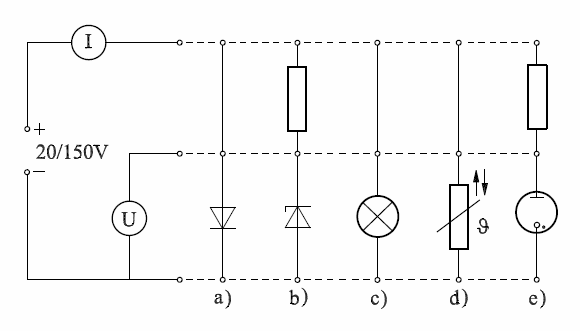
\includegraphics[width=\textwidth]{Versuch1.png}
			\caption{Schaltskizze zu Versuch 1}
			\label{Schaltskizze1}
		\end{figure}

		\subsection{a) Diode in Durchlassrichtung} 
			\label{a)}
			
			\subsubsection*{Diode}
				\label{Diode}
								
				Eine Diode ist ein Bauteil, durch das elektrische Ströme nur in eine Richtung durchgelassen werden.
				Diesen Effekt erhält man, wenn man einen Halbleiter mit einem Element aus der dritten Hauptgruppe (p-Leiter) und einen anderen mit einem Element aus der fünften Hauptgruppe (n-Leiter) dotiert und diese aneinander grenzen lässt.
				Hierbei entsteht eine Raumladungszone im Übergangsbereich, da die Elektronen des n-Leiters zu dem p-Leiter wandern.
				Da in diesem Übergangsbereich weniger freie Ladungsträger sind, als im restlichen Leiter, nimmt die Leitfähigkeit stark ab.
				
				Wird eine äußere Spannung angelegt, bei der der positive Pol auf den n-Leiter trifft, so vergrößert sich der Übergangsbereich.
				Bei Umkehrung der Polung hingegen, verkleinert sich dieser und verschwindet bei ausreichend hoher Spannung komplett, sodass der Strom durch den Leiter fließen kann. 
			
			\subsubsection*{Messung}
				
				Die Messwerte sind in Abb. \ref{KL a} zu sehen. Die Kennlinie verläuft bei dieser Diode in Durchflussrichtung exponentiell.
				Ein messbarer Strom wurde erst ab ca. \SI{0.5}{\V} erhalten und es ließen sich ab ungefähr \SI{0.72}{\V} keine weiteren Werte messen. Höhere Spannungen konnten durch Regulierung an der Spannungsquelle nicht erreicht werden. Im Bereich \SIrange{0,65}{07}{\V} wurde das Einstellen besonders schwierig.
				
				\begin{figure}
					\centering
					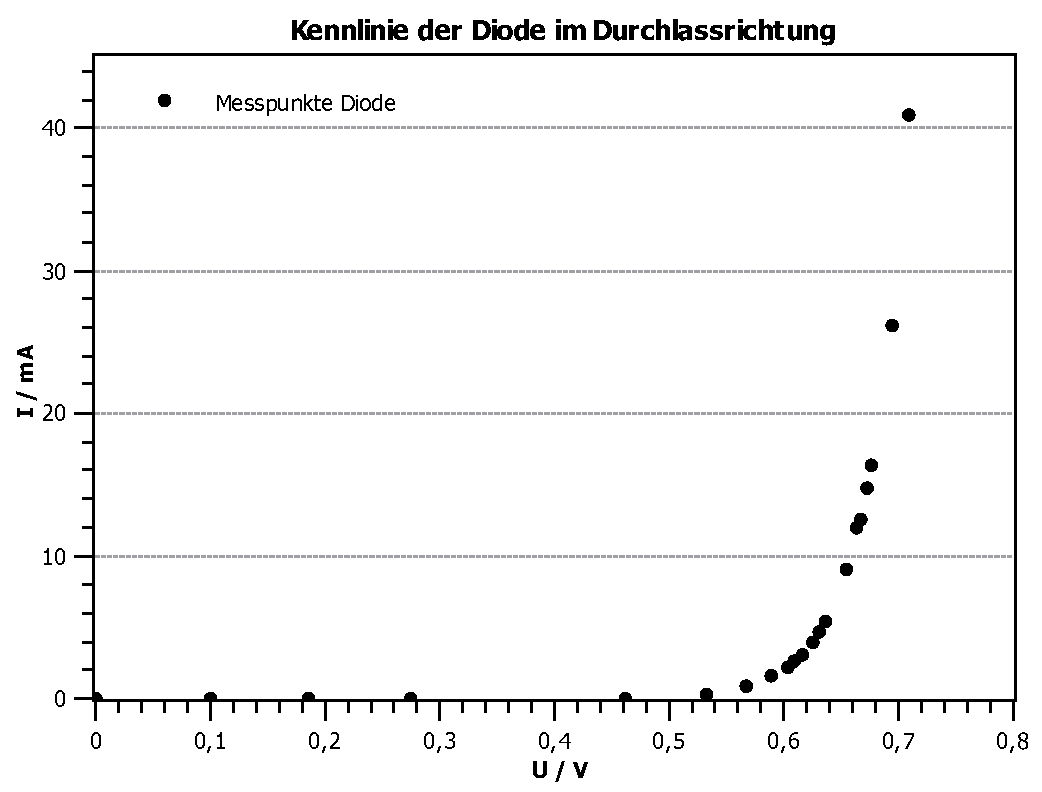
\includegraphics[width=\textwidth]{KennlinieDiode.pdf}
					\caption{U-I-Kennlinie einer Diode in Durchlassrichtung}
					\label{KL a}
				\end{figure}
			
			\subsubsection*{Einordnung der Ergebnisse}
							
				Die Ergebnisse deuten darauf hin, dass mindestens \SI{0.5}{\V} nötig sind, um den Übergangsbereich der Diode soweit zu verkleinern, dass überhaupt ein Strom fließen kann. 				
				Dass sich ab ca. \SI{0.72}{\V} keine weiteren Werte messen  ließen, lag daran, dass keine höheren Eingangsspannungen möglich waren. Hierbei könnte der Innenwiderstand des Netzteils, sowie weitere Vorwiderstände eine Rolle spielen.

				Die Größe des Übergangsbereichs steht in direktem Zusammenhang mit dem Widerstandswert der Diode.
				Denn bei einer höheren Spannung ist auch der Übergangsbereich kleiner und freie Ladungsträger können leichter passieren.
				Der Widerstand wird demnach geringer.
				
				Dieser Sachverhalt wird durch den exponentiellen Verlauf der ermittelten Kennlinie unterstützt.
				Das Ergebnis entspricht somit den Erwartungen.
				
		\subsection{b) Zenerdiode} 
			
			Die Zenerdiode funktioniert ähnlich wie die in \ref{Diode} beschriebene Diode, nur dass bei dieser der elektrische Strom auch in Sperrrichtung fließen kann.
			Ursache dafür ist die geringe Größe der Potentialbarrieren bei hochdotierten p-n-Übergängen, wenn hohe Spannungen angelegt werden.
			Hierbei kommt es zu dem quantenmechanischen Tunneleffekt, durch welchen Valenzelektronen in das Leitungsband gelangen.
			Es fließt ein Durchbruchstrom, welcher die Diode nicht zerstört, wie es bei einem Lawinendurchbruch der Fall wäre.
			
			\subsubsection*{Messung}
			
				 \begin{itemize}
				 	
				 	\item Sperrrichtung: 
				 	
				 	Auch in Abb. \ref{KL b1} ist ein exponentieller Verlauf der Kennlinie zu erkennen.
				 	Anders als in der vorausgehenden Messung, fließt hier jedoch erst ab ca. \SI{2.6}{\V} ein Strom, welcher sich dieses mal bis ungefähr \SI{5}{\V} messen ließ.
				 	Damit liegt die Durchbruchspannung deutlich über der Durchlassspannung.
				 	
				 	\begin{figure}
				 		\centering
				 		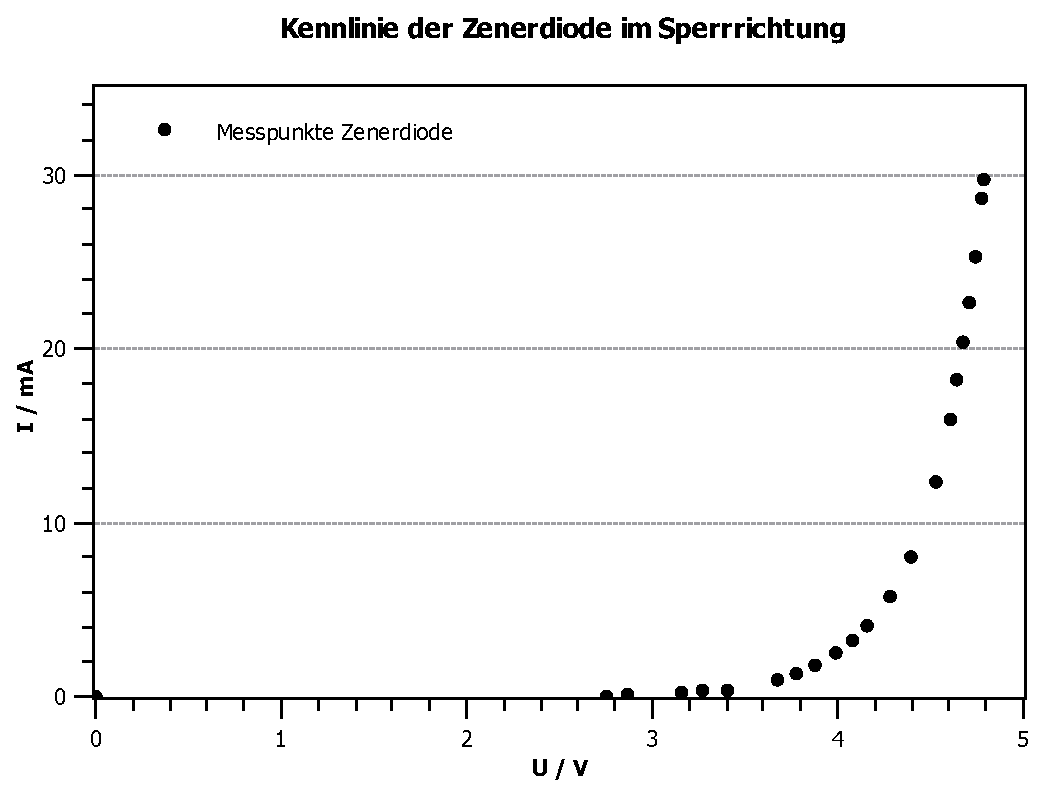
\includegraphics[width=\textwidth]{KennlinieZenerdiodeSperrrichtung.pdf}
				 		\caption{U-I-Kennlinie einer Zenerdiode in Sperrrichtung}
				 		\label{KL b1}
				 	\end{figure}
				 	
				 	\item Durchlassrichtung:  
				 	
				 	Diese Messung verlief analog zu der in \ref{a)} durchgeführten Messung, wie in Abb. \ref{KL b2} zu sehen.
				 	Auch hier beträgt die Durchlassspannung ca. \SI{0,55}{\V}.

				 	Verglichen mit Abb. \ref{KL a}, ist diese gleichmäßiger und der zu erkennende exponentielle Anstieg wirkt minimal stärker.
				 	
				 	\begin{figure}
				 		\centering
				 		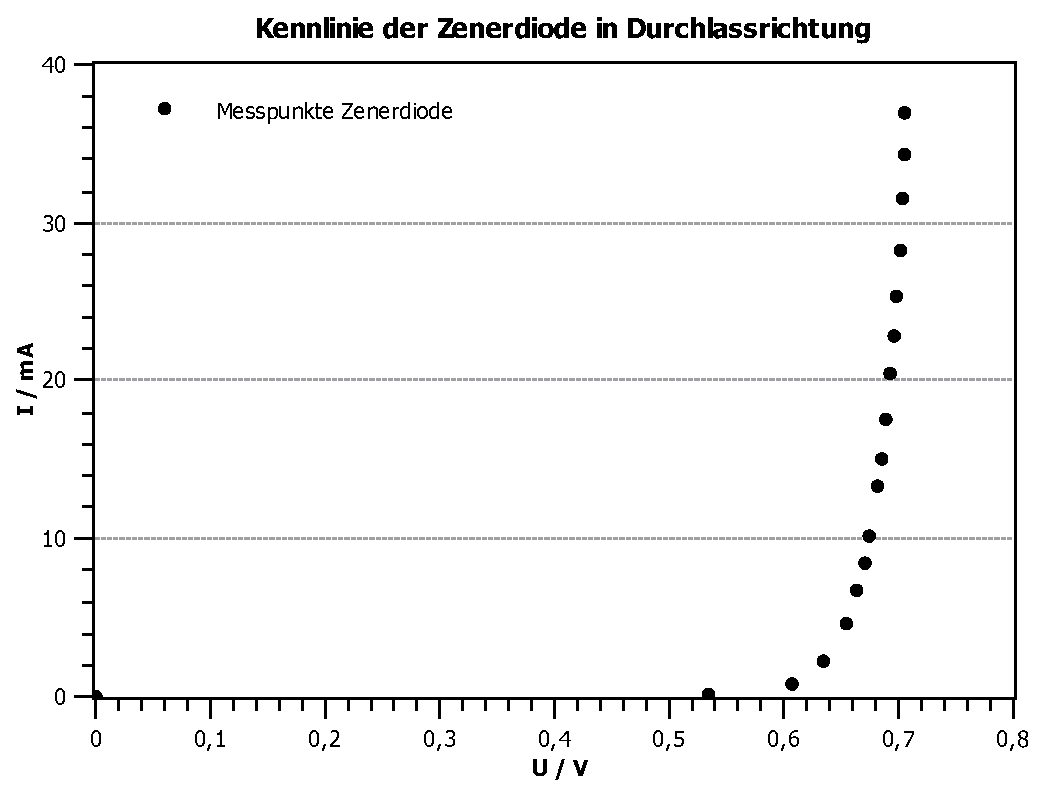
\includegraphics[width=\textwidth]{KennlinieZenerdiodeDurchlassrichtung.pdf}
				 		\caption{U-I-Kennlinie einer Zenerdiode in Durchlassrichtung}
				 		\label{KL b2}
				 	\end{figure}
				 					 	
				\end{itemize}
											
			\subsubsection*{Einordnung der Ergebnisse}
				
				Die Ergebnisse dieser Messung bezüglich der Durchlassrichtung stehen in direktem Zusammenhang zu dem Ergebnis aus \ref{a)}. 
				Für die Sperrrichtung hingegen wurde ermittelt, dass die benötigte Spannung für einen Stromfluss bei ca. \SI{2.6}{\V} liegt. 
				
				Verglichen mit den \SI{0.5}{\V} in Durchflussrichtung ist dies ein beachtlicher und zu erwartender Unterschied.
				Im Gegenzug zu der Verkleinerung des Übergangsbereichs der Diode fließt in Sperrrichtung, wenn überhaupt, nur der Durchbruchstrom und für diesen benötigt man hohe Spannungen. 
				
				Dass auch in Sperrrichtung die Kennlinie exponentiell verläuft, hat einen ähnlichen Grund, wie in Durchflussrichtung.
				Denn mit höheren Spannungen lösen sich auch mehr Elektronen aus dem Valenzband des p-Leiters und folglich ist der Durchbruchstrom stärker.
				Der Widerstandswert wird also auch hier mit höherer Spannung kleiner. 
				
		\subsection{c) Glühlampe} 
			
			Bei der Glühlampe fließt der Strom durch einen Glühdraht. Dieser erwärmt sich dabei und beginnt zu glühen. Es wird betrachtet, wie sich der Widerstand der Glühlampe in Abhängigkeit von der Spannung ändert. Dazu wird der Strom wie bisher gemessen und gegen die Spannung aufgetragen.
			Um die Änderung des Widerstandes besser zu betrachten, wird dieser gegen die Spannung aufgetragen. 
			
			\subsubsection*{Messung}
				
				Die Kennlinie der Glühlampe verläuft zunächst logarithmisch, richtet sich im späteren Verlauf jedoch annähernd linear aus. Es lässt sich beobachten, dass die Glühlampe ab ca. \SI{2.6}{\V} anfängt schwach zu glühen. In Abb. \ref{KL c} ist zu sehen, dass die Kennlinie beginnt sich in diesem Bereich linear auszurichten.
				Der Graph in Abb. \ref{R c} zeigt, dass auch ohne angelegte Spannung, also bei Zimmertemperatur, ein Widerstand vorliegt. Der weitere Verlauf ist annähernd linear, wobei sich die Steigung bei ca. \SI{2}{\V} ändert (kleiner wird).
				
				Der letzte messbare Wert lag hier bei ca. \SI{7.2}{\V}.
				
				\begin{figure}
					\centering
					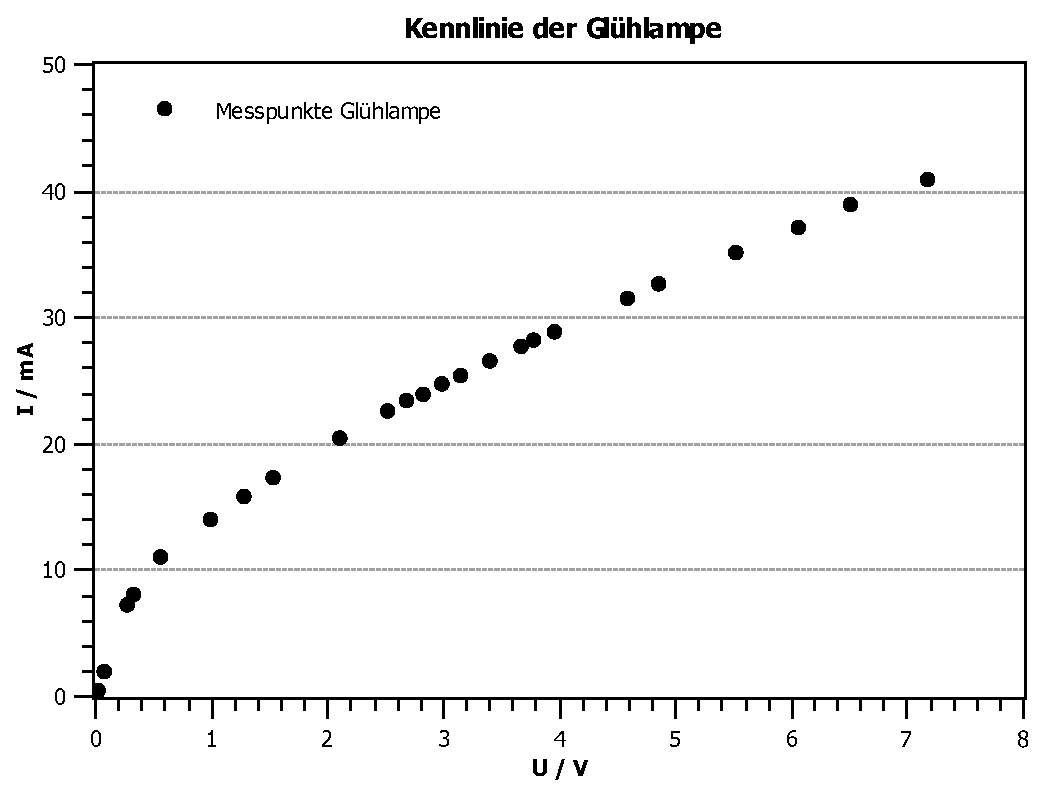
\includegraphics[width=\textwidth]{KennlinieGluehlampe.pdf}
					\caption{U-I-Kennlinie einer Glühlampe}
					\label{KL c}
				\end{figure}
				\begin{figure}
					\centering
					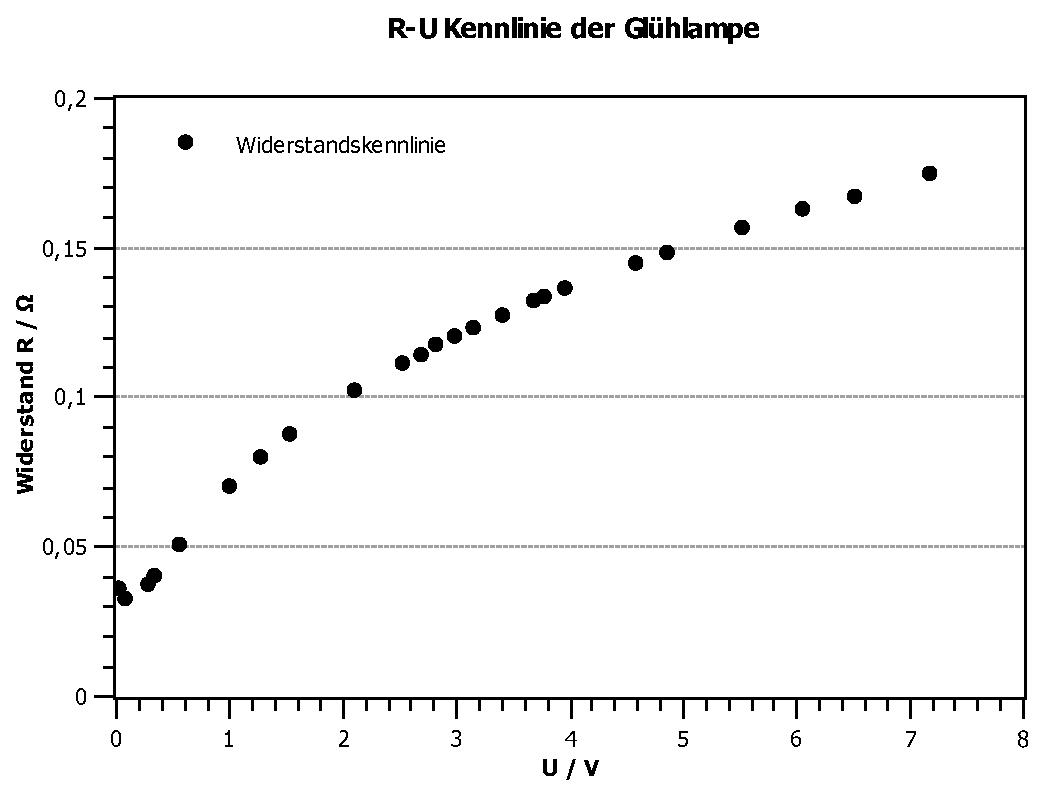
\includegraphics[width=\textwidth]{KennlinieGluehlampeWiderstand.pdf}
					\caption{R-U-Kennlinie einer Glühlampe}
					\label{R c}
				\end{figure}
			
			\subsubsection*{Einordnung der Ergebnisse}
						
				Der annähernd lineare Verlauf der Kennlinie bei Spannungen ab ca. \SI{2.6}{\V} deutet darauf hin, dass der Widerstand sich bei höheren Spannungen weniger ändert.
				In Abb. \ref{R c} ist zu erkennen, dass dies der Fall ist, wobei der Widerstand weiterhin langsam steigt.
				
				Das allgemeine Steigen des Widerstands lässt sich auf die steigende Temperatur zurückführen.
				Bei dem Glühdraht handelt es sich um ein Metall, vermutlich Wolfram.
				Metalle haben die Eigenschaft, dass ihre elektrische Leitfähigkeit mit steigender Temperatur abnimmt.
				
				Zu Beginn ist der Glühdraht bei Zimmertemperatur und wie in Abb. \ref{R c} zu erkennen ist, steigt der Widerstand zunächst stark an, weswegen die Kennlinie erst logarithmisch verläuft.
				Ab dem Punkt, an dem der Draht glüht, steigt der Widerstand langsamer, da die Temperaturunterschiede schwächer werden.
				
				Durch Linearisierung der Messwerte zwischen \SI{0}{\V} und \SI{2}{\V} ist zu erkennen, dass der y-Achsenabschnitt, also der Widerstand bei Zimmertemperatur, bei ca. \SI{25}{\Omega} liegt.
				
				Dieses Verhalten stimmt mit der Änderung der elektrischen Leitfähigkeit von Metallen bei erhöhten Temperaturen überein.
				
		\subsection{d) NTC-Widerstand} 
			
			NTC-Widerstände bestehen aus Halbleitern und verhalten sich, was den Widerstand betrifft, anders als Metalle.
			Das \glqq NTC\grqq{} steht für \glqq Negative Temperature Coefficient\grqq{}, da sie bei erhöhten Temperaturen, im Gegensatz zu Metallen, den elektrischen Strom besser leiten als bei geringeren Temperaturen. Diese bezeichnet man als Warmleiter.
			
			Bei dieser Messung wird ein NTC-Widerstand untersucht.
			Vor dem Aufnehmen eines jeden Messwertes wird der Widerstand zwei bis drei Minuten in Ruhe gelassen, damit sich ein Temperaturgleichgewicht einstellen kann.
			
			\subsubsection*{Messung}
			
				In Abb. \ref{KL d} ist ähnlich zu den Dioden ein exponentiellen Verlauf der Kennlinie zu erkennen, wobei dieser Widerstand von Anfang an den Strom durchlässt und nicht erst ab einer gewissen Spannung.
				Hier konnten nur Werte bis $U = \SI{8}{\V}$ Eingangsspannung aufgenommen werden.
				
				\begin{figure}
					\centering
					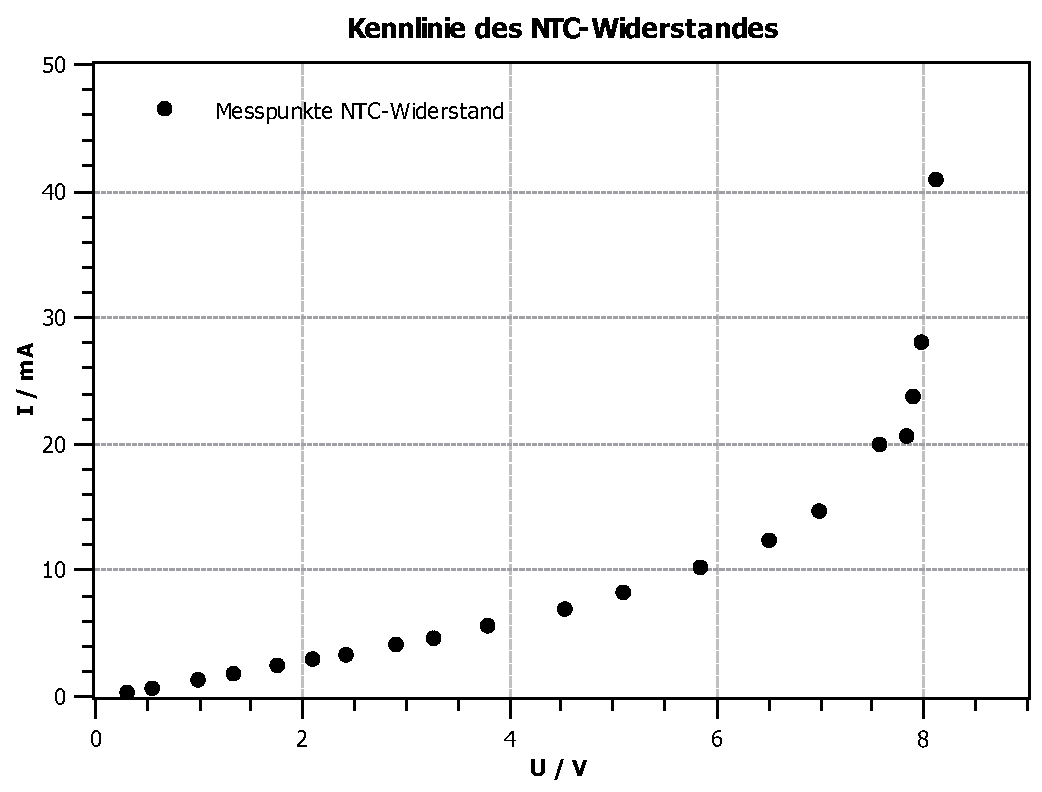
\includegraphics[width=\textwidth]{KennlinieNTCsubgitter.pdf}
					\caption{Messung zu Versuch 1d)}
					\label{KL d}
				\end{figure}
			
			\subsubsection*{Einordnung der Ergebnisse}
			
				Hier ist klar zu erkennen, dass der Widerstand mit steigender Temperatur (durch steigende Ströme) sinkt, was für NTC-Widerstände charakteristisch ist. 
				Dass sich auch hier keine höheren Eingangsspannungen als \SI{8}{\V} einstellen ließen, könnte ebenfalls an dem Innenwiderstand des Netzteils gelegen haben.
			
		\subsection{e) Glimmlampe} 
			
			Bei der Glimmlampe kann der Strom nicht einfach durchfließen, da kein elektrischer Leiter die beiden Pole direkt miteinander verbindet.
			Damit ein Strom fließen kann, müssen freie Ladungsträger, also Ionen und Elektronen, von der Kathode zur Anode gelangen.
			Zwischen den beiden befindet sich lediglich ein Gas, in dem sich die freien Ladungsträger bewegen können. Gasentladungen sind nötig, damit die Ladungen diese Strecke passieren können.
			
			\subsubsection*{Gasentladungen}
			
				Die anliegende Spannung setzt Elektronen aus der Kathode frei.
				Je höher die anliegende Spannung, desto stärker werden die Elektronen beschleunigt und erreichen bei der Anode eine höhere Maximalgeschwindigkeit und somit eine höhere kinetische Energie, jedoch geringere potentielle Energie.
				Sind die Elektronen schnell genug um die Gasatome durch Stoßionisation zu ionisieren, so folgt eine Kettenreaktion von sich lösenden Elektronen.
				Die Spannung, welche man für die Ionisation der Gasatome braucht, nennt man Zündspannung. 
				
				An der Anode kommen schließlich aus den Gasatomen gelöste Elektronen an und ein Strom fließt, solange die Ionisation des Gases aufrecht erhalten wird.
				Sinkt die Spannung unter die sogenannte Löschspannung, dann ist dies nicht mehr möglich und der Stromfluss wird unterbrochen.

				Die Löschspannung ist geringer als die Zündspannung, da nur noch für die Anregung Energie benötigt wird und dafür weniger notwendig ist, als für die Ionisation der Gasatome.
					
				Zudem wird Licht bei der Ionisation des Gases bzw. dem Zurückfallen der Elektronen emittiert, was das \glqq Glimmen\grqq{} der Lampe ausmacht.
				
			\subsubsection*{Messung}
			
				Zunächst wird gemessen, welche Zündspannung notwendig ist, um die Glimmlampe zu zünden.
				Für diese Spannung wurde ein Wert von ca. \SI{119}{\V} gemessen.
				Danach fiel die gemessene Eingangsspannung schnell auf ca. \SI{88,4}{\V} ab und es ließ sich nun ein Strom messen.
				Hier fing die Glimmlampe auch an zu leuchten.
				Bis zum Erreichen der Zündspannung war der Strom gleich null, weswegen nur der relevante Bereich in Abb. \ref{KL e} dargestellt ist.
				
				Bis zu ca. \SI{92}{\V} ließ sich die Eingangsspannung erhöhen. In diesem Bereich sieht das Strom-Spannungs-Verhältnis nahezu linear aus.
				
				Das Herunterregeln der Eingangsspannung ergab unerwartete Effekte. Wie zum Beispiel, dass es teilweise zu höheren Spannungen an der Glimmlampe geführt hat, was zu dem Verlauf der Messpunkte in Abb. \ref{KL e} führte.				
				Der Strom hingegen wurde mit dem Herunterregeln kleiner bis schließlich eine Stromstärke von null erreicht wurde\footnote{siehe dazu Reihenfolge der Messwerte im Laborbuch, Seite 2}.

				Nachdem die Glimmlampe erloschen war, musste die angelegte Spannung wieder bis zur Zündspannung erhöht werden, um sie zu entzünden.
			
				\begin{figure}
					\centering
					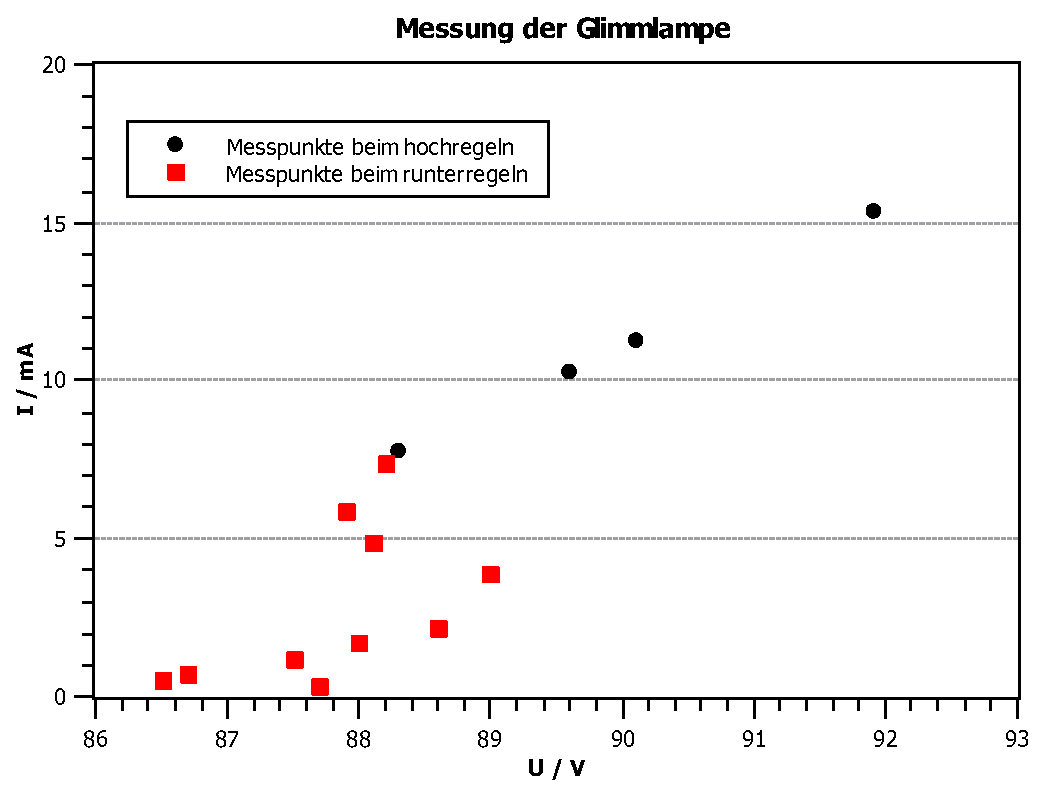
\includegraphics[width=\textwidth]{KennlinieGlimmlampe.pdf}
					\caption{U-I-Kennlinie einer Glimmlampe}
					\label{KL e}
				\end{figure}
			
			\subsubsection*{Einordnung der Ergebnisse}
			
				Der Messung lässt sich entnehmen, dass die Zündspannung der Glimmlampe bei ca. \SI{119}{\V} liegt.
				
				Die Löschspannung liegt zwischen \SI{86,5}{\V} und \SI{88}{\V}. Sie konnte nicht eindeutig festgelegt werden, da zwar bei \SI{87,7}{\V} die Lampe erlischt, es jedoch auch niedrigere Spannungen gab, bei denen die Lampe noch geleuchtet hat.
				
				Für die Zündspannung wurde uns ein Wert von ungefähr \SI{120}{\V} vorgegeben, welcher mit unserer Messung weitgehend übereinstimmt, lediglich eine Differenz von \SI{1}{\V}.
					
	\newpage	
	\section{Versuch 2: Widerstand in Abhängigkeit der Temperatur}		
		
		Dieser Versuch beschäftigt sich mit der Leitfähigkeit eines Kupferdrahtes in Abhängigkeit der Temperatur.
		
		\subsection{Methoden} 
		
			Der Kupferdraht wird in eine Wheatstone'sche Brückenschaltung integriert (siehe Abb. \ref{Schaltskizze2}). Hierbei bezeichnet $R_\text{x}(T)$ den Kupferdraht, $R_\text{v}$ einen einfachen \SI{5}{\Omega}-Widerstand und $R_\text{e}$ den \SI{11,3}{\Omega} Widerstand, welcher sich wie ein Potentiometer einstellen lässt. Bei diesem handelt es sich um einen Schiebewiderstand. Widerstände dieser Art sind proportional zur Länge $l$ des Metalls und antiproportional zur ihrer Querschnittsfläche $A$. 
			
			\begin{equation*}
				R = \varrho \frac{l}{A} \Rightarrow R_e(x) = \frac{x}{l} R_0 = \SI{11,3} x \cdot \si{\Omega\per\meter}
			\end{equation*}				
			$x$ sei hierbei die Position des Schiebereglers und $l$ die gesammte Länge des Drahtes.	
			
			Das Prinzip der Wheatstone'schen Brücke ermöglicht mit Hilfe der Kirchhoff'schen Regeln einen unbekannten Widerstand zu berechnen.
			Wird an dem Strommessgerät, wie es in Abb. \ref{Schaltskizze2} verbaut ist, kein Strom gemessen, dann gilt nach dem Abgleichverfahren
			\begin{equation*}
				\frac{R_e(x)}{R_0-R_e(x)} = \frac{R_\nu}{R_x} \Rightarrow R_x = \frac{x}{l-x} R_\nu.
			\end{equation*}
			Der Widerstand $R_\text{e}$ über den Schieberegler wird für jede Messung so eingestellt, dass $I = \SI{0}{\A}$ erfüllt wird. Es wird erst über den \SI{20}{k\Omega} kalibriert und dann über den geschlossenen Schalter für genauere Messungen.
			
			Vor Beginn der Messung, wird der Draht auf ca. \SI{0}{\celsius} abgekühlt.
			Nun wird er langsam auf nahezu \SI{100}{\celsius} erhitzt und währenddessen kontinuierlich die Temperatur und die Position des Schiebereglers gemessen.
			Das Gleiche wird für die Abkühlung bis \SI{15}{\celsius} wiederholt.
						
			\begin{figure}
				\centering
				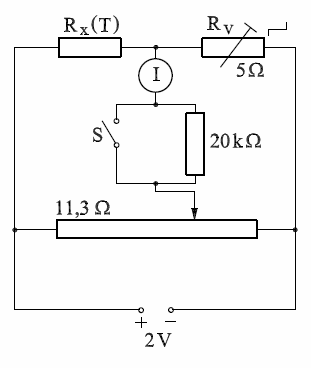
\includegraphics[width=0.6\textwidth]{Versuch2.png}
				\caption{Schaltskizze zu Versuch 1}
				\label{Schaltskizze2}
			\end{figure}
		
		\subsection{Messung}
			
			Die Gesamtlänge des Drahts liegt bei \SI{100}{cm}. In Abb. \ref{fig:drahtRT} sind die umgerechneten Widerstände gegen die Temperatur aufgetragen. Die Ausgleichsgerade hat eine Steigung von $m = \SI{0,021335}{\Omega\per\celsius}$ und schneidet die y-Achse bei $y_0 = \SI{5,005}{\Omega}$.
			
			\begin{figure}
				\centering
				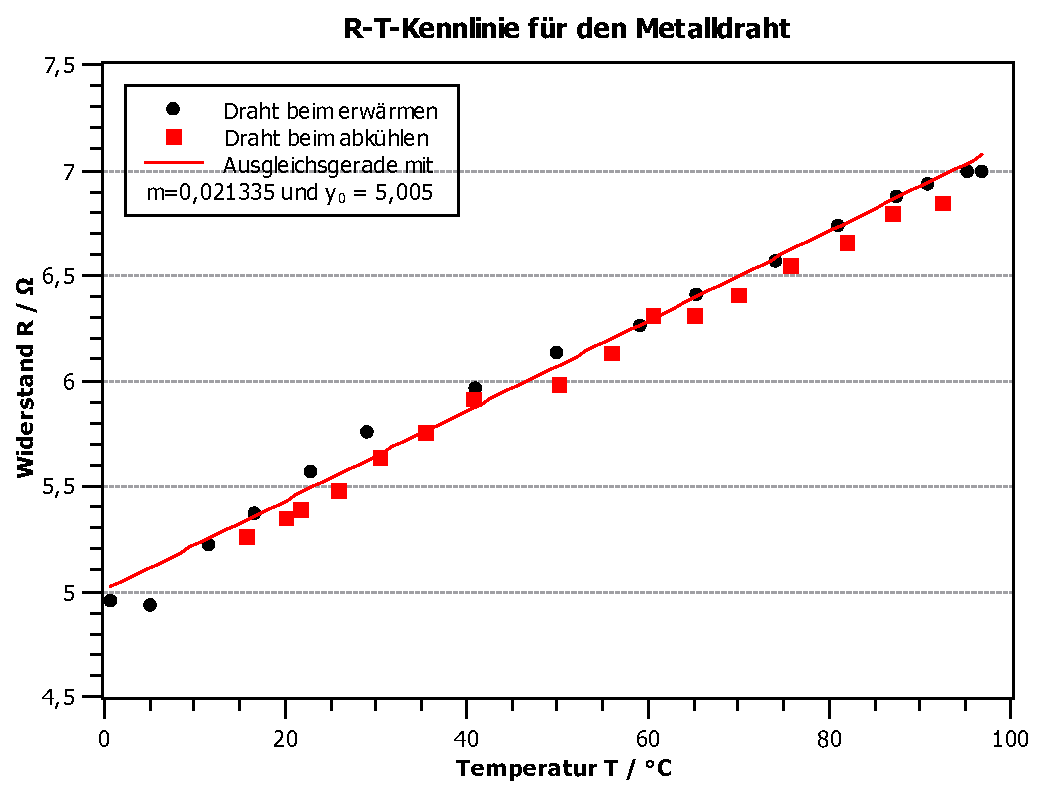
\includegraphics[width=\textwidth]{KennlinieDrahtRT.pdf}
				\caption{Widerstand des Drahtes relativ zur Temperatur}
				\label{fig:drahtRT}
			\end{figure}
			
		\subsection{Einordnung der Ergebnisse}	
			
			Der Widerstand des Drahtes steigt wie erwartet mit zunehmender Temperatur. 
			Entgegen der Erwartung jedoch ist der Widerstand des Drahtes nicht vorgelaufen, sondern eher zurückgeblieben.
			Das ist in Abb. \ref{fig:drahtRT} gut daran zu erkennen, dass die meisten Werte beim Erwärmen über der Geraden liegen, während sie beim Abkühlen größtenteils unter dieser sind.
			
			Der Temperaturkoeffizient $\alpha$ entspricht:
			\begin{equation*}
				\alpha = \frac{R(T)-R_\text{Raum}}{R_\text{Raum}\cdot (T-T_\text{Raum})} \approx \SI{0,00426}{\K^{-1}}
			\end{equation*} 
			Verglichen mit dem Literaturwert für Kupfer von \SI{0,00393}{\K^{-1}}, weicht dieser um 8,4\% ab. Eine genauere Messung wäre demnach angebracht.
			Der y-Achsenabschnitt $y_0$ ist der Widerstand bei $T=\SI{0}{\celsius}$, also $R_x(T=\SI{0}{\celsius}) = \SI{5,005}{\Omega}$.
		
	\begin{thebibliography}	{}
		Die Abbildungen \ref{Schaltskizze1} und \ref{Schaltskizze2} wurden der Versuchsanleitung entnommen
	\end{thebibliography}	
			
\end{document} 